\scanpage{122}
% archive sheet number: 121

corps et si on se borne aux modules de type fini sur $k$, on est dans les conditions de 6), et on trouve le groupe algébrique $\underline{G}_m$ sur $k$. D'ailleurs même sans condition sur $k$ et sans se borner à des modules de type fini, on récupère $C$ avec toutes ces structures par les représentations de $\underline{G}_m$\handwritten{\unsure{!|/|.}}

Gardons $\otimes$, $\handwritten{\phi}$ (et $\underline{1},u,v$) comme dessus, mais changeons $\handwritten{\unsure{\psi|\mu}}$ \deleted{ou $\handwritten{\unsure{\phi|\psi}}$}, en \deleted{\unsure{tri}} utilisant la règle de Koszul. Ce\inserted{\handwritten{nouveau}} choix de $\handwritten{\mu}$ s'impose dans certaines questions. Par exemple supposons $k$ un corps, \deleted{de car. nulle,} soit $V$ la catégorie des espaces topologiques compacts, avec le foncteur $\otimes$ donné \unsure{par} produit cartésien, et la donnée évidente d'associativité et de commutativité (pour le c\deleted{\unsure{a}}oup on n'a vraiment pas le choix !); il y a\deleted{\unsure{x}} une unité, \unsure{à} savoir l\deleted{\unsure{es}}'espace\deleted{s} ponctuel. Considérons le foncteur cohomologique $X\handwritten{\mapsto}H^{\handwritten{\bullet}}(X,k)$ sur $V^{\unsure{o|0}}$, utilisant Künneth on trouve un isomorphisme $c$ de compatibilité aux $\otimes$\inserted{de $V^o$ dans $C$}. Ce dernier est compatible aux structures a),b),c) \uline{à condition} de choisir $\handwritten{\mu}$ dans $C$ par la règle de Koko\deleted{\unsure{f}}!

A prouver que lorsque on prend $C$comme dessus à la Koko, il n'y\deleted{\unsure{a}} a pas de foncteur fibre sur $C$ sur aucune extension $K$ de $k$ (même en\deleted{\unsure{s}} se bornant aux vectoriels de dim\unsure{e|m}nsion finie) !

% Thin separation stroke between C and comme in the preceding paragraph.
\figure{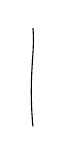
\begin{tikzpicture}[baseline]\draw (0,-.55) .. controls (-.06,.1) and (.03,.4) .. (0,.7);\end{tikzpicture}}

\margin{???}
\margin{\figure{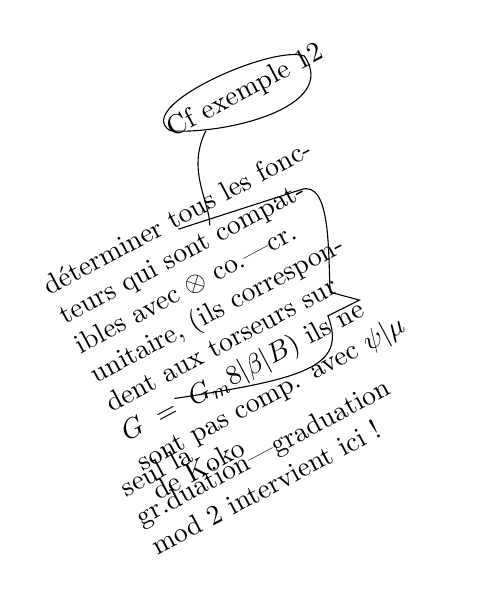
\begin{tikzpicture}[baseline]
\node[rotate=28] at (1.05,4.9) {\handwritten{Cf exemple 12}};
\draw (.1,4.4) .. controls (-.4,4.7) and (1.4,5.5) .. (1.8,5.35) .. controls (2.25,4.7) and (.8,4.35) .. (.1,4.4);
\draw (.55,4.4) .. controls (.3,3.9) and (.6,3.5) .. (.6,3.2);
\draw (.2,3.15)--(1.75,3.65) .. controls (2.15,3.8) and (2.1,2.8) .. (2.13,2.35)--(2.5,2.25)--(2.1,2.05) .. controls (2.35,1.4) and (1.8,1.25) .. (.15,1.0);
\node[rotate=28,align=left,text width=4.2cm] at (1.05,2.1) {\handwritten{déterminer tous les foncteurs qui sont compatibles avec $\otimes$ \unsure{co.|cr.} unitaire, \unsure{(}ils correspondent aux torseurs sur $G=G_m\unsure{8|\beta|B}$) \uline{ils ne sont pas comp. avec $\unsure{\psi|\mu}$ de Koko}}};
\node[rotate=28,align=left,text width=3.9cm] at (1.4,.4) {\handwritten{seul la \unsure{gr.duation|graduation} mod $2$ intervient ici !}};
\end{tikzpicture}}}

Pour pallier à cet inconvénient, il y a lieu\deleted{\unsure{lorsqu'on s'en va dans} une \unsure{catégori|catégorie} avec $\otimes$ la catégorie des} d\deleted{\unsure{e}}'étudier systématiquement les $\otimes$-foncteurs compatibles avec a)b)c) à valeurs dans une catégorie\inserted{de modules \unsure{grad|gradués}} $\mathbb{C}$ comme ci-dessus: ce sont \handwritten{l}es\handwritten{``}\uline{foncteurs fibres tordus}\handwritten{''}. En particulier, si $C$ est comme au début de 6) (pas encore de $\otimes$), supposons que le foncteur $F$ se factorise (de façon donnée) par les modules gradués, i.e. qu'on ait un foncteur compatible avec les foncteurs oublis $C\handwritten{\to}\mathrm{Gradf}(k)\unsure{=|\equiv}\mathbb{D}^{\unsure{\mathbb{X}|X}}$. Cela correspond à un homomorphisme de coalgèbres de $A$ dans $k\handwritten{[}T,T^{-1}\handwritten{]}$; où à la donnée d'éléments $\handwritten{\pi}_i$ de $U$ (les projections sur les composants homogènes) satisfaisant les conditions \deleted{$\unsure{\handwritten{\pi}_i=0_i|\handwritten{\pi}_i\pi_i=0}$} habituelles
